\chapter{Visual Scalability }
\label{chap:scalability}
The visual exploration of large time-oriented data in business creates new requirements for visualizations. We describe these in this chapter. One of these requirements - the scalability of time-oriented visualization techniques - is determined by assessing the \hyperref[databasemetrics]{database metrics} and visualization characteristics of time-oriented visualization techniques. As visualization techniques alone are not sufficient however, data reduction and interaction techniques are discussed to define further criteria for visual scalable tools.

\section{Database Metrics} \label{databsemetrics}
The maximum number of rows which can be managed by a tool influences the tool's visual scalability. While creating a visualization the user loads a data set with its corresponding size - large sized in the context of our work - into the tool's backend. Due to technical reasons tools restrict the number of rows either during the data load from the database into the tool (backend) or during the data load from the tool into the visualization (frontend). In the second case visualizations are restricted in the number of rows for visualizations even if the available number of rows in the backend is higher. The characteristic of the maximal number of rows during data load in the backend or frontend is one possibility to define a \textit{database metric}. In the context of large data visualization, database metrics are a determining factor for scalability. Sometimes tools limit the initial number of rows and the user has to write additional code to extend the maximum row number. This affects the ease-of-use negatively.

\section{Visual Scalability of Time-Oriented Techniques}\label{visualization}
The visualization characteristics are determined by the choice of the visualization technique.
% introduction of methodology: selection of vizTechniques, introduction of classes
The selection of the visualization technique greatly influences the scalability, as illustrated by the following example. 
A line chart maps one dimension to the x-axis while a second dimension is mapped to the y-axis as in figure \ref{fig:linechart}. Considering that each data item requires one screen pixel along the y-axis to be displayed, the maximum number of data items is limited by the monitor width. 
\begin{figure}[H]
    \centering
    \scalebox{0.2}{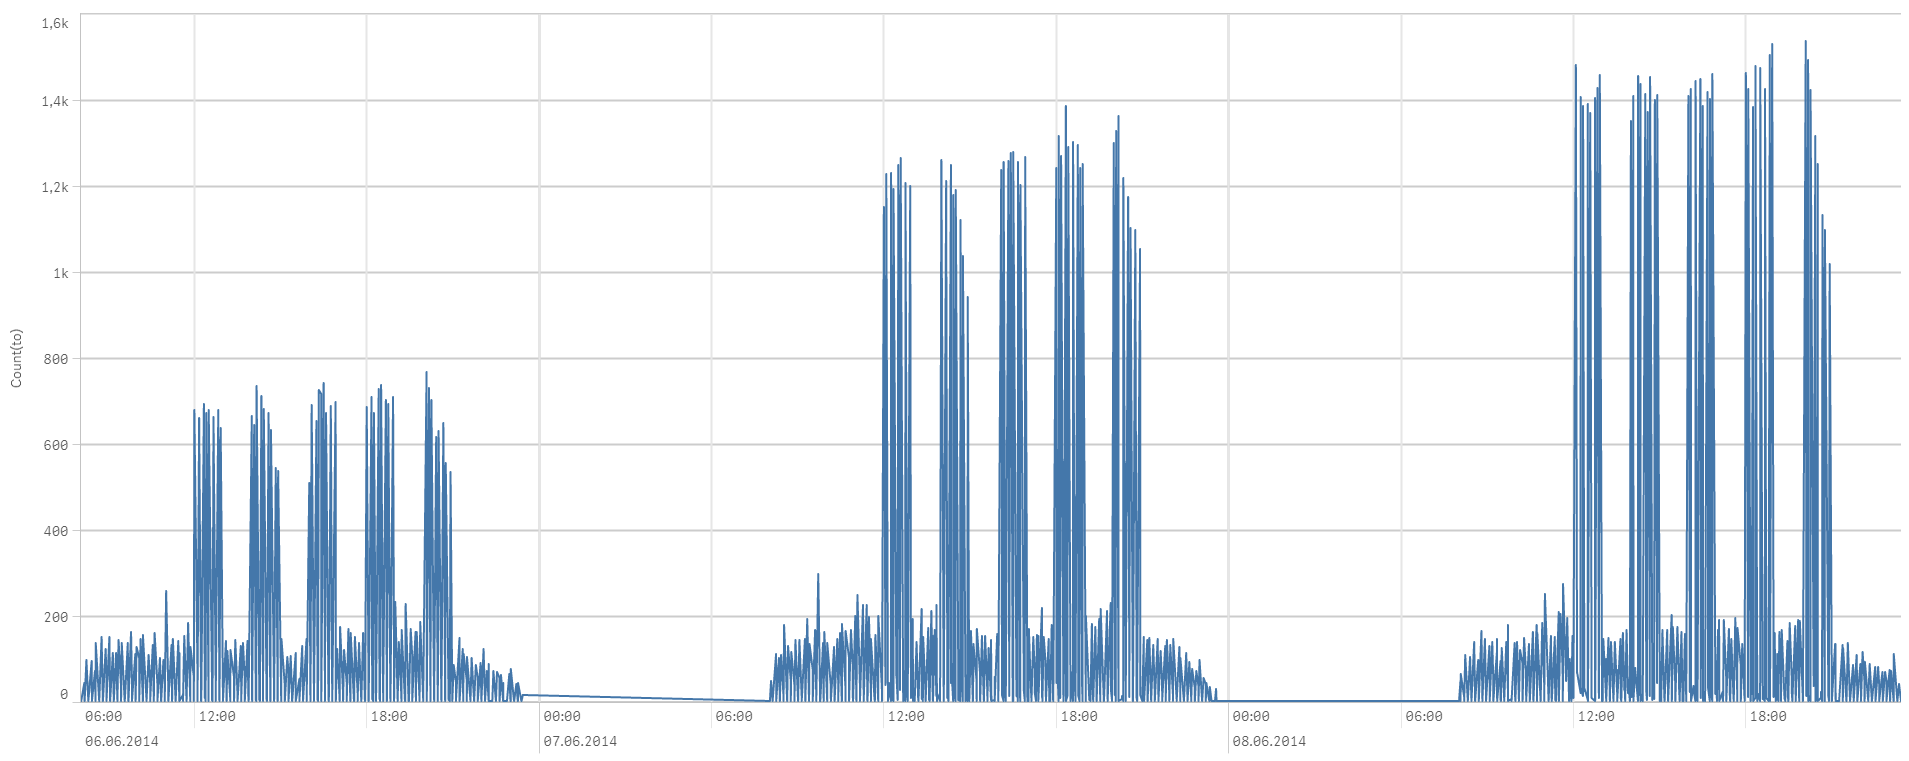
\includegraphics{src/images/linechart}}
    \caption[Line Chart]{Line Chart}
    \label{fig:linechart}
\end{figure}
 
In contrast, the scatter plot can use up to  five attributes\footnote{The five attributes are x-position, y-position, form, shape, size.} so the maximum number of displayable data items in the scatter plot exceeds the maximum in the line chart. While the line chart in \ref{fig:linechart} shows the count of one dimension along the time-axis \ref{fig:scatterplot} maps the count of two dimensions along the time. Hence, the scatter plot shows more information and is more scalable.
\begin{figure}[H]
    \centering
    \scalebox{0.2}{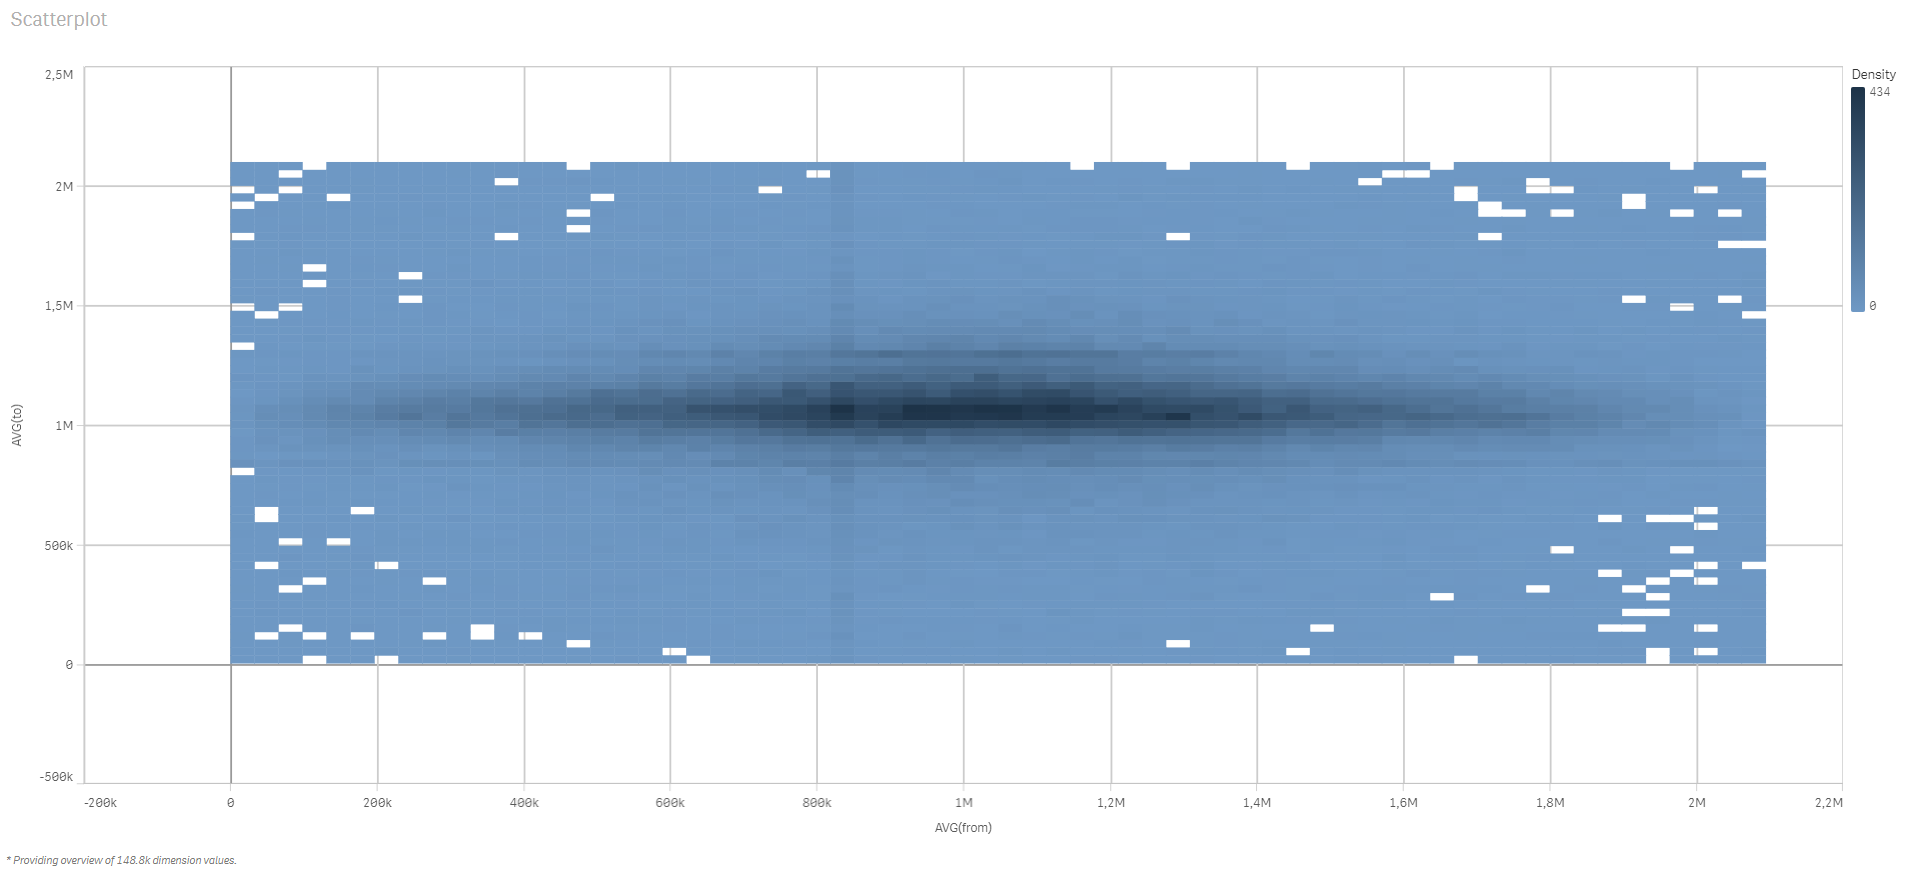
\includegraphics{src/images/SmartDataCompression}}
    \caption[Scatter Plot]{Scatter Plot}
    \label{fig:scatterplot}
\end{figure}

For this work we selected time-oriented visualization techniques for multivariate data (\ref{vis}). Our selection of time-oriented techniques can be classified into four of Keim's visualization classes: geometric, hierarchical, icon-based and pixel-oriented. In table \ref{table:vizScalability} to \ref{table:vizScalabilityPixel} we categorized each technique into one of the four classes based on the techniques' visual metaphor and discussed the classes' scalability.

\begin{table}[H]
	\centering
	\caption [Geometric-Projective techniques]{ Geometric-Projective techniques (\gls{GP})}
	\label{table:vizScalability}
	\begin{tabular}{| l | l | l |}
	\hline
	\rowcolor{gray!30}Visualization Class & Technique & References\\
	\hline
	    \multirow{8}*{Geometric} 
		& EventRiver        &  \cite{Luo2012}\\
		& Flocking Boids    &  \cite{Moere2004}\\
	    & Kiviat Tube       &  \cite{Tominski2005}\\
        & MultiComb         &  \cite{Tominski2004}\\
        & Multi-resolution CircleView &  \cite{Keim2005}\\
        & Parallel Glyphs   &  \cite{Fanea2005}\\
        & Temporal Star     &  \cite{Noirhomme-Fraiture2002}\\
        & TimeWheel         &  \cite{Tominski2004}\\ \hline
        \end{tabular}
\end{table}
        Geometric-Projective techniques (\gls{GP}) try to find a interesting projection to map multi-dimensional data to the 2D screen  \cite{FerreiradeOliveira2003}.
        The visualization characteristics of \gls{GP} strongly depend on the mapping-function that regulates the projection. The mapping-function often includes data reduction techniques (see section \ref{analytical}).  When data reduction techniques are involved, this class of techniques is able to visualize large to huge data sets. This class will be described in detail (\ref{GP-Techniques}).
        
\begin{table}[H]
	\centering
	\caption[Hierarchical Techniques]{Hierarchical Techniques}
	\label{table:vizScalabilityHierarchical}
    \begin{tabular}{| l | l | l |}
	\hline
    \rowcolor{gray!30}Visualization Class & Technique & References\\
	\hline
		\multirow{3}*{Hierarchical} 
		& Pixel-Oriented Network Visualization  &  \cite{Stein2013}\\
		& Software Evolution Analysis   &  \cite{Gall1999}\\
		& Timeline Trees                &  \cite{Burch2008}\\ \hline
\end{tabular} 
\end{table}
        Hierarchical techniques subdivide the screen into $k$ subsets. 
		We analyzed three hierarchical visualization techniques. Timeline Trees include aggregation techniques by collapsing the tree nodes. With collapsed nodes the technique can display large to huge amounts of data. Pixel-oriented Networks use clustering via which similar time lines are visually grouped together. All hierarchical visualizations scale to more than two million pixels.
		
\begin{table}[H]
	\centering
	\caption[Icon-based Techniques]{Icon-based Techniques}
	\label{table:vizScalabilityIcon}		
    \begin{tabular}{| l | l | l |}
	\hline
    \rowcolor{gray!30}Visualization Class & Technique & References\\
	\hline
        \multirow{5}*{Icon-based}
        & Gravi++       & \cite{Hinum2005}\\
        & InfoBUG       & \cite{Chuah1998}\\
        & PeopleGarden  & \cite{Xiong1999}\\
        & Spiral Graph  & \cite{Weber2001}\\
        & VIE-VISU      & \cite{Horn2001}\\ \hline
\end{tabular} 
\end{table}

        As every data item requires one icon, icon-based techniques can show less data items than the number of pixels on the screen. When showing large data, icon-based techniques face the challenge of clutter and occlusion \cite{Borgo2013}. Thus, icon-based techniques can only display small- to medium-sized data sets.
        
\begin{table}[H]
\centering
\caption[Pixel-Oriented Techniques]{Pixel-Oriented Techniques}
\label{table:vizScalabilityPixel}
\begin{tabular}{  | l | l | l |}
	\hline
    \rowcolor{gray!30}Visualization Class & Technique & References\\
	\hline
        \multirow{12}*{Pixel-oriented}
        & 3D ThemeRiver &  \cite{Imrich2002}\\
        & Braided Graph &  \cite{Javed2010}\\
        & CircleView    &  \cite{Keim2005}\\
        & Data Tube Technique &  \cite{Ankerst2001}\\
        & history flow  &  \cite{Viegas2004}\\
        & Kaleidomaps   &  \cite{Bale2007}\\
        & Pixel-Oriented Network Visualization  &  \cite{Stein2013}\\
        & Recursive Pattern &  \cite{Keim1995}\\
        & Spiral Display    &  \cite{Carlis1998}\\
        & Stacked Graphs    &  \cite{Byron2008}\\
        & ThemeRiver        &  \cite{Havre2000}\\
        & Time Curves       &  \cite{Bach2016}\\
        & TimeRider         &  \cite{Rind2011}\\ \hline
\end{tabular}
\end{table}

        Since only one pixel per data item is used, this class can maximize the used screen space. Let $M$ be the monitor resolution with the screen-width $w$ and the screen-height $h$, $P$ the number of pixels in $M$ and $D$ the maximum of data which can be displayed at once. In pixel-oriented techniques  \begin{math}
        D = w*h
        \end{math}
        which shows that pixel-oriented techniques can display large, but not huge data. Assuming a monitor resolution with two million pixels, the scalability is up to two million pixels.

% \thispagestyle{empty}
% \begin{table}[H]
% 	\centering
% 	\caption[Visualization Classes]{Visualization Classes}
% 	\label{table:vizScalability}
% 	\begin{tabular}{  | l | l | l |}
% 	\hline
% 	\rowcolor{gray!30}Visualization Class & Technique & References\\
% 	\hline
% 	    \multirow{8}*{Geometric} 
% 		& EventRiver        &  \cite{Luo2012}\\
% 		& Flocking Boids    &  \cite{Moere2004}\\
% 	    & Kiviat Tube       &  \cite{Tominski2005}\\
%         & MultiComb         &  \cite{Tominski2004}\\
%         & Multi-resolution CircleView &  \cite{Keim2005}\\
%         & Parallel Glyphs   &  \cite{Fanea2005}\\
%         & Temporal Star     &  \cite{Noirhomme-Fraiture2002}\\
%         & TimeWheel         &  \cite{Tominski2004}\\ \hline
%         \multicolumn{3}{|p{\linewidth}|}{
%         The visualization characteristics of Geometric-Projective techniques (\gls{GP}) strongly depend on the mapping-function that regulates the projection of multi-dimensional data to the 2D screen  \cite{FerreiradeOliveira2003}. The mapping-function often includes data reduction techniques (see section \ref{analytical}).  When data reduction techniques are involved, this class of techniques is able to visualize large to huge data sets. This class will be described in detail (\ref{GP-Techniques}).} \\ \hline
        
% 		\multirow{3}*{Hierarchical} 
% 		& Pixel-Oriented Network Visualization  &  \cite{Stein2013}\\
% 		& Software Evolution Analysis   &  \cite{Gall1999}\\
% 		& Timeline Trees                &  \cite{Burch2008}\\ \hline
% 		\multicolumn{3}{|p{\linewidth}|}{We analyzed three hierarchical visualization techniques. Timeline Trees include aggregation techniques by collapsing nodes. With collapsed nodes the technique can display large to huge amounts of data. Pixel-oriented Networks use clustering via which similar time lines are visually grouped together. Hierarchical visualizations scale to more than two million pixels.} \\ \hline
%         \multirow{5}*{Icon-based}
%         & Gravi++       & \cite{Hinum2005}\\
%         & InfoBUG       & \cite{Chuah1998}\\
%         & PeopleGarden  & \cite{Xiong1999}\\
%         & Spiral Graph  & \cite{Weber2001}\\
%         & VIE-VISU      & \cite{Horn2001}\\ \hline
%         \multicolumn{3}{|p{\linewidth}|}{
%         As every data item requires one icon, icon-based techniques can show less data items than the number of pixels on the screen. When showing large data, icon-based techniques face the challenge of clutter and occlusion \cite{Borgo2013}. Thus, icon-based techniques can only display small- to medium-sized data sets.}\\ \hline
%         \multirow{12}*{Pixel-oriented}
%         & 3D ThemeRiver &  \cite{Imrich2002}\\
%         & Braided Graph &  \cite{Javed2010}\\
%         & CircleView    &  \cite{Keim2005}\\
%         & Data Tube Technique &  \cite{Ankerst2001}\\
%         & history flow  &  \cite{Viegas2004}\\
%         & Kaleidomaps   &  \cite{Bale2007}\\
%         & Pixel-Oriented Network Visualization  &  \cite{Stein2013}\\
%         & Recursive Pattern &  \cite{Keim1995}\\
%         & Spiral Display    &  \cite{Carlis1998}\\
%         & Stacked Graphs    &  \cite{Byron2008}\\
%         & ThemeRiver        &  \cite{Havre2000}\\
%         & Time Curves       &  \cite{Bach2016}\\
%         & TimeRider         &  \cite{Rind2011}\\ \hline
%         \multicolumn{3}{|p{\linewidth}|}{
%         Since only one pixel per data item is used, this class can maximize the used screen space. Let $M$ be the monitor resolution with the screen-width $w$ and the screen-height $h$, $P$ the number of pixels in $M$ and $D$ the maximum of data which can be displayed at once. In pixel-oriented techniques  \begin{math}
%         D = w*h
%         \end{math}
%         which shows that pixel-oriented techniques can display large, but not huge data.}
%         \\ \hline
% 	\end{tabular}
% \end{table}

The scalability and visualization characteristics at the same time are summarized in table \ref{table:vizScalabilityOverview}. 

\begin{table}[H]
	\centering
	\caption[Scalability of Visualization Classes]{Scalability of Visualization Classes}
	\label{table:vizScalabilityOverview}
	\begin{tabular}{ l | c }
	\hline
	Visualization Class & Scalability\\
	\hline
	Geometric &  \cellcolor{green!25 } > 2 mio. pixel\\
	Hierarchical & \cellcolor{green!25} > 2 mio. pixel \\
	Icon-based & \cellcolor{red!25} $\leq$ 1 mio. pixel \\
	Pixel-oriented & \cellcolor{yellow!25} $\leq$ 2 mio. pixel \\	
	\hline
	\end{tabular}
\end{table}

Table \ref{table:vizScalabilityOverview} shows that most of the existing visualization techniques may visualize large data up to two million data items but they are not appropriate in visualizing huge data. Pixel-based visualizations represent each data item by one pixel and thus, are limited to the monitor resolution. Even new visualization techniques which where developed to visualize "very large" data sets follow the pixel-oriented approach. Icon-based visualizations display one data item per icon and thus can display even less data than pixel-oriented visualization techniques. The most promising techniques are hierarchical and geometric-projective techniques, as they combine aggregation with visualization. Their scalability depends on the mapping-function. 
One interesting extension of pixel-oriented techniques is the \textit{multi-resolution} approach  \cite{Keim2005} which is described in detail in \ref{multi-resolution}.







%Aspects of Scalability:
% Wie viele Datenpunkte sind notwendig, um Pattern darzustellen? -> data 
% Interaction Techniques
% Downsampling -> Analytical Methods
% \iffalse
%  The challenges of large-scale data for \gls{ADV} are \textit{scalability} and \textit{dynamics}  \cite{Wang2015}. With its volume the challenges for large-scale data are also challenges for Big Data defined as high volume, high velocity, high veracity and high variety data sets  \cite{Wang2015}. In this work we concentrate on the scalability challenge for visualization techniques. The challenge is in finding appropriate techniques  \cite{Aigner2008,Keim2005} which scale to large amount of data.
 
% \fi

\subsubsection{Visualization characteristics of \gls{GP}} \label{GP-Techniques}
Geometric-projective visualizations together with hierarchical techniques are the most scalable visualization technique depending on the mapping function. For this reason we will explore techniques in the geometric-projective class in detail and discuss their scalability.


Furthermore, we suggest to divide \gls{GP} into \textit{radial} and \textit{non-radial} visualizations (compare table \ref{table:radialTable}) to determine their visual scalability. The literature review has shown that a large part of \gls{GP} is based on a radial layout. Radial \gls{GP} share common properties such as the maximum number of attributes which is set to 10-20 attributes  \cite{Diehl2010}. The number of attributes is needed in measuring the number of distinct items to determine the visualization characteristics of \gls{GP}. Therefore, the number of distinct items is equal to the maximum number of data items times the maximum number of attributes.\par


\begin{table}[H]
	\centering
	\caption[Radial and non-radial \gls{GP}]{Radial and non-radial \gls{GP}}
	\label{table:radialTable}
	\begin{tabular}{lcc}
	\hline
	\gls{GP}-Technique & radial & non-radial \\
	\hline
	Flocking Boids &  & x \\
	Kiviat Tube & x &  \\
	MultiComb & x &  \\
	Multi-resolution CircleView & x &  \\
	Parallel Glyphs & x &  \\
    Temporal Star & x &  \\
	TimeWheel & x & \\
	\hline
	\end{tabular}
\end{table}


\textbf{Flocking Boids} (figure \ref{fig:flockingboids}) simulate the evolution of data items in 3D. Thus, data objects are represented by a colored, curved line with changing transparency called \textit{boid}.  A data object is an aggregation of equal data items, e.g. one boid is one stock market company. A boid calculates the average of multiple data attributes and uses behavior rules to simulate the development of a data object. The rules define the position of a data item over time as well as its velocity. Time is represented by animation and boids correspond to distinct items on the screen. Therefore the maximum measured number of used boids defines the scalability. Flocking boids are able to handle 500 boids at a time. Thus the scalability of Flocking Boids is 500 which is low compared to pixel-oriented techniques (two million items)  \cite{Moere2004}.
Analytical methods such as clustering or subset selection are outsourced to database algorithms and interaction techniques are not implemented but could be extended \cite{Moere2004}. 
\begin{figure}[H]
    \centering
        \scalebox{.5}{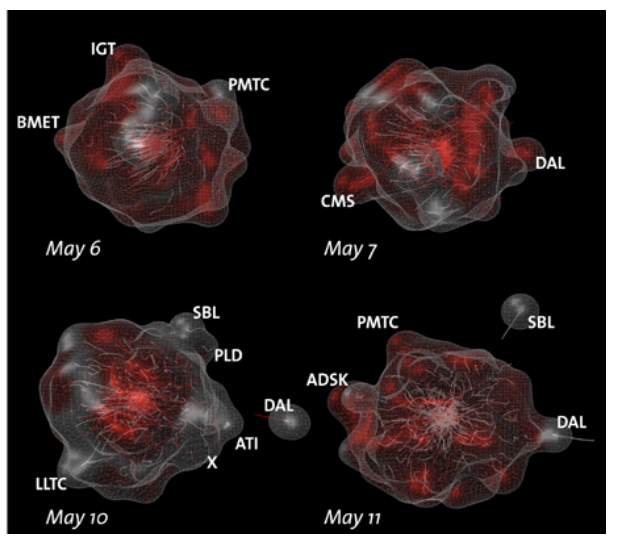
\includegraphics{src/images/FlockingBoids}}
    \caption[Flocking Boids]{Flocking Boids. From  \cite{Aigner2011}.}
    \label{fig:flockingboids}
\end{figure}
\par
\textbf{Kiviat Tube} (figure \ref{fig:kiviattube}) is an unfolded Radar Chart along the z-axis in 3D. Several Radar charts are stacked along the time (z) axis and form a tube. Thus, variables are mapped on radial aligned planes and can be compared. Interaction such as changing the plane's positions and navigating through time enables the user to compare different variables over time.
\par
The number of attributes is limited to approximately 10-20 attributes as the radial layout limits the number of variables. Since the Kiviat Tube is a 3D representation, the tube is projected to the 2D screen. Let $w$ be the window width. Then, the maximum number of data items is $\leq w$ as the technique does not include any aggregation. The scalability is $20*w\approx 20.000$.
\begin{figure}[H]
    \centering
        \scalebox{.5}{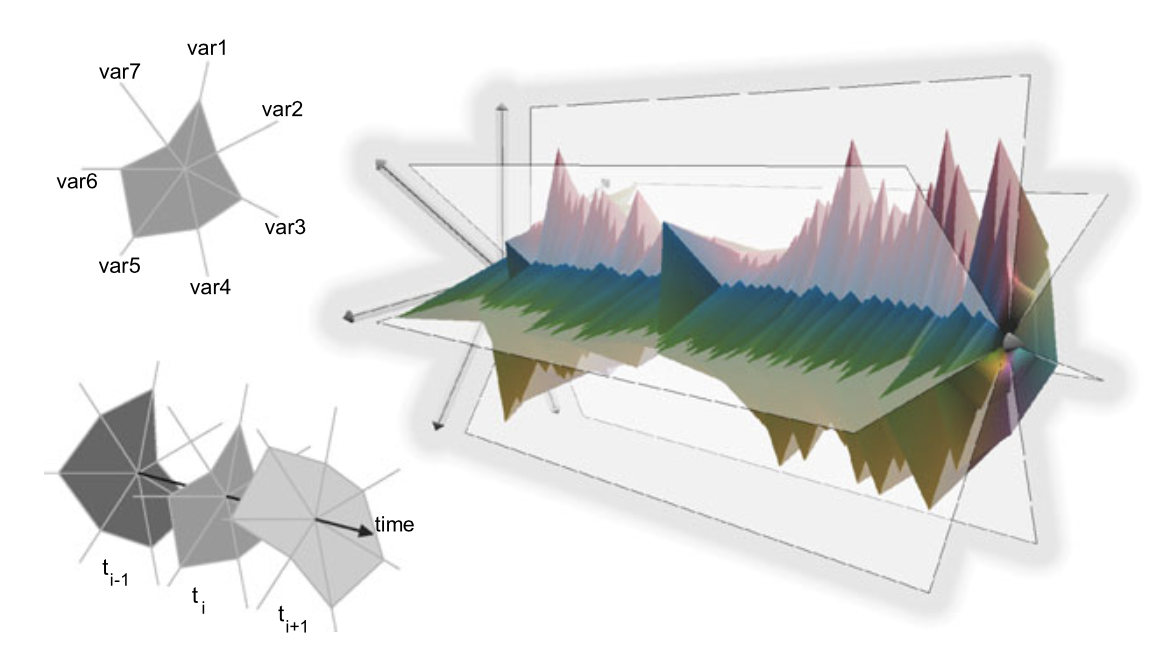
\includegraphics{src/images/KiviatTube}}
    \caption[Kiviat Tube]{Kivit Tube. From  \cite{Aigner2011}.}
    \label{fig:kiviattube}
\end{figure}
\par
In \textbf{MultiComb} (figure \ref{fig:multicomb}) \textit{k} time series plots are mapped on a circle in two possible ways. One way is to position the plots along the circumference. The other is to map the plots perpendicularly to the circumference. In this version the plot resembles a star.  The MultiComb is radial. Let $h$ be the window height, then the maximum number of data items in version two is $< \frac{h}{2}$ and the scalability $20*< \frac{h}{2} \approx 10.000$
\begin{figure}[H]
    \centering
        \scalebox{.5}{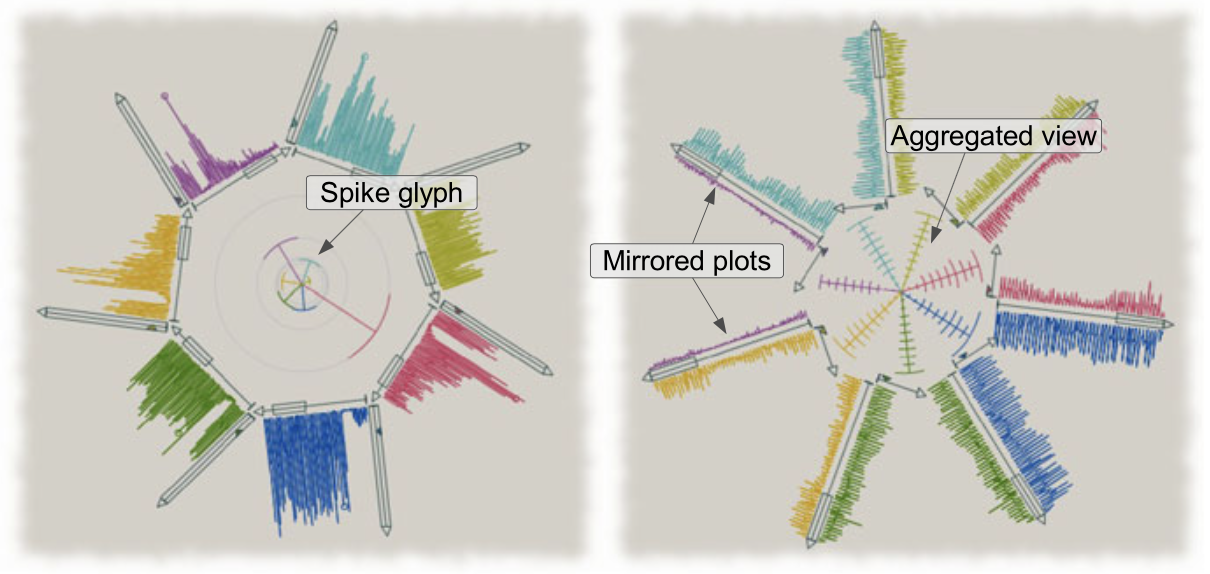
\includegraphics{src/images/MultiComb1,2}}
    \caption[Multi Comb]{Multi Comb. From  \cite{Luo2012}.}
    \label{fig:multicomb}
\end{figure}
\par
\textbf{Multi-resolution CircleView} (figure \ref{fig:multiresolutioncircleview}) enhances the CircleView technique. Instead of mapping each value to one pixel, data items are aggregated. More recent items are placed in the middle of the circle. These items are represented by one pixel each. Less relevant items are aggregated and placed at the outer part of the circle. These items are usually from a preceding point of time. Since Multi-resolution CircleView uses aggregation, the maximum number of data items is $> 2mio.$ pixels, which makes Multi-resolution CircleView a scalable visualization.
\begin{figure}[H]
    \centering
        \scalebox{.5}{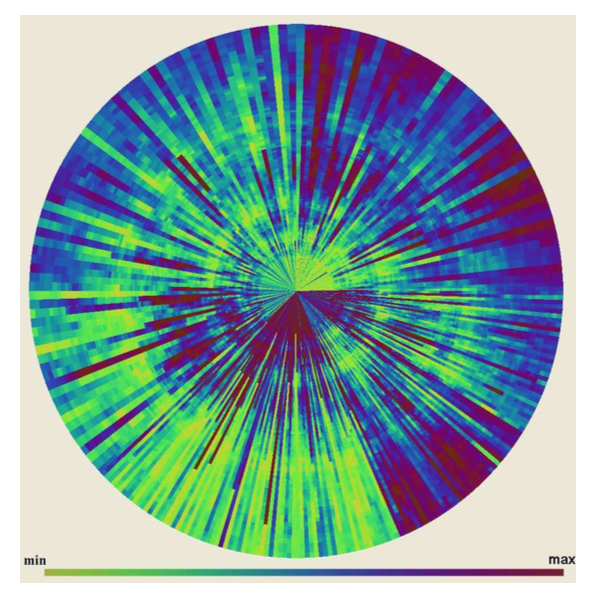
\includegraphics{src/images/MultiResolutionCircleView}}
    \caption[Multi-Resolution CircleView]{Multi-resolution CircleView. From  \cite{Keim2005}.}
    \label{fig:multiresolutioncircleview}
\end{figure}
\par
\textbf{Parallel Glyphs} (figure \ref{fig:parallelglyphs}) pair parallel coordinates with Star Glyphs. While similar to parallel coordinates each data item is represented by a polyline that connects the vertical axis (attributes). The attribute axis are radially unfolded in 3D and show the data value of the data item over time. Thus, each data value over time is represented by a star glyph. The visualization can be expanded by connection lines over star glyphs. Parallel Glyphs provide brushing of polylines, filtering, axis reordering, rotating in three directions,  transparency support if the glyphs overlap each other, and the presentation of focus-and-context through magnification lenses. Through the extension of 2D to 3D parallel glyphs are able to display more data rows than parallel coordinates (\gls{PC}). \gls{PC} have the problem of clutter while displaying 15.000 data items on a gray-scale  \cite{Keim2000Tut}. However, as the maximum number of data items is below one million data points, parallel glyphs are not a scalable visualization technique. 

\begin{figure}[H]
    \centering
        \scalebox{.4}{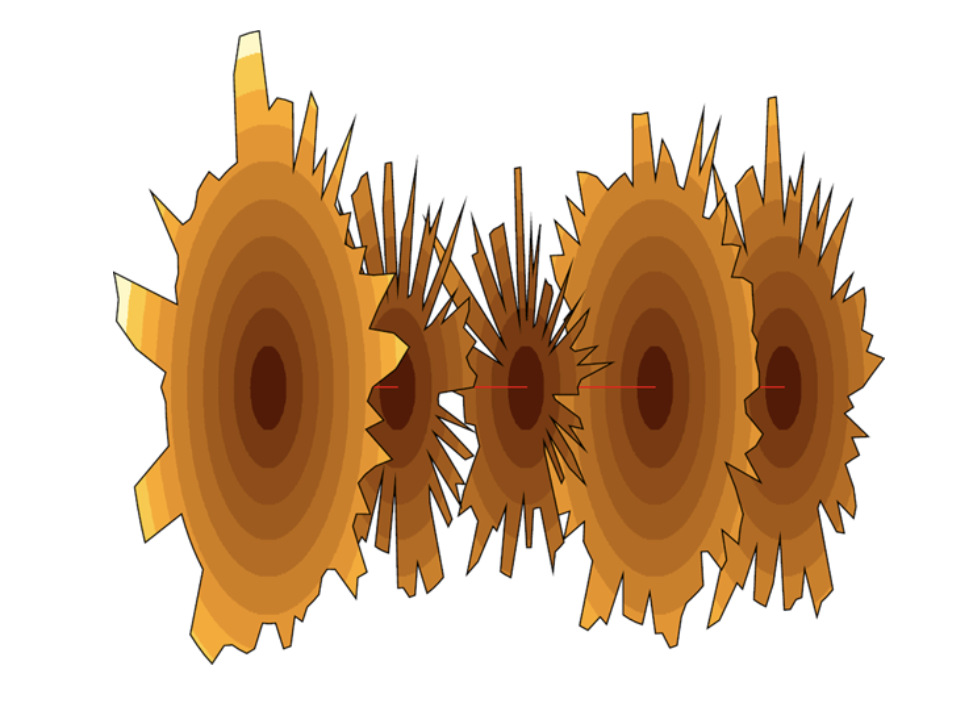
\includegraphics{src/images/ParallelGlyphs}}
    \caption[Parallel Glyphs]{Parallel Glyphs. From  \cite{Aigner2011}.}
    \label{fig:parallelglyphs}
\end{figure}\par

\textbf{Temporal Star} (figure \ref{fig:temporalstar}) aligns multiple attributes in a star-like manner around the centre. Each star is one point of time. The time axis connects several stars to a 3D-object. A temporal star uses so-called \textit{symbolic objects} to display aggregated data. With 10 - 20 attributes and aggregated data items, temporal stars are designed to show large data sets. 
\begin{figure}[H]
    \centering
        \scalebox{.5}{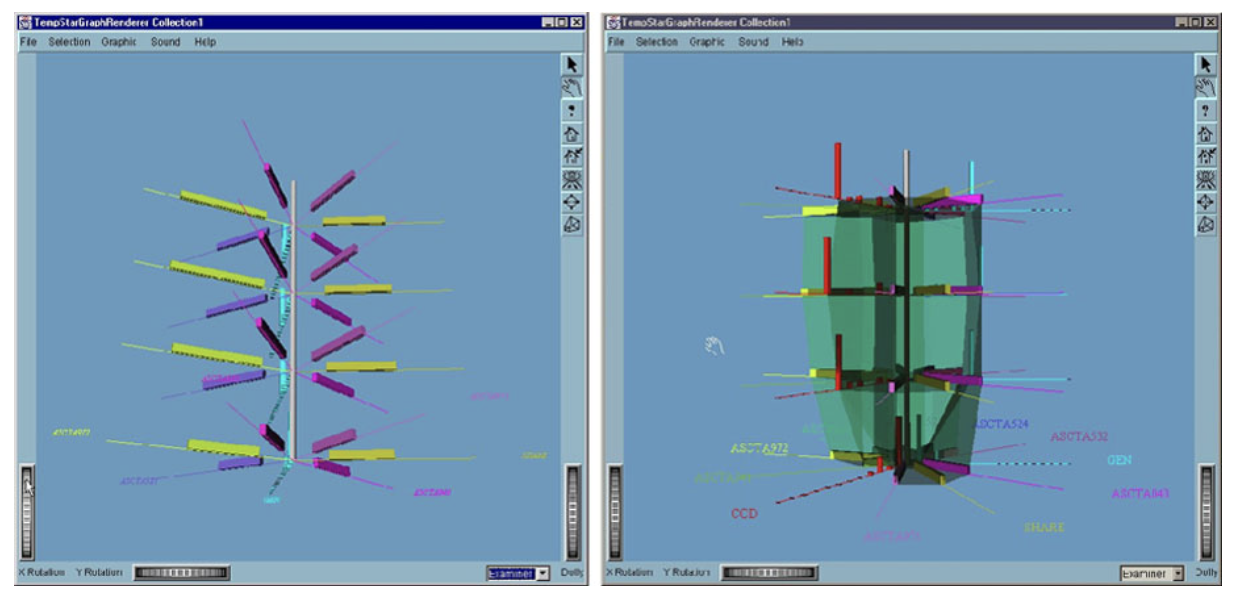
\includegraphics{src/images/TemporalStar}}
    \caption[Temporal Star]{Temporal Star. From  \cite{Aigner2011}.}
    \label{fig:temporalstar}
\end{figure}\par

\textbf{TimeWheel} (figure \ref{fig:timewheel}) is a 2D technique. Similar to the first variation of the \textit{MultiComb}, the attribute axes are positioned along the circle circumference. In the centre of the circle the time axis is placed. Let $a$ be the pixel width of this axis and $a < w$. Similar to the MultiComb method, a TimeWheel does not include aggregation and thus the maximum number of data items is limited to $a$. Thus, the scalability is $20* a \approx 10.000$.
\begin{figure}[H]
    \centering
        \scalebox{.5}{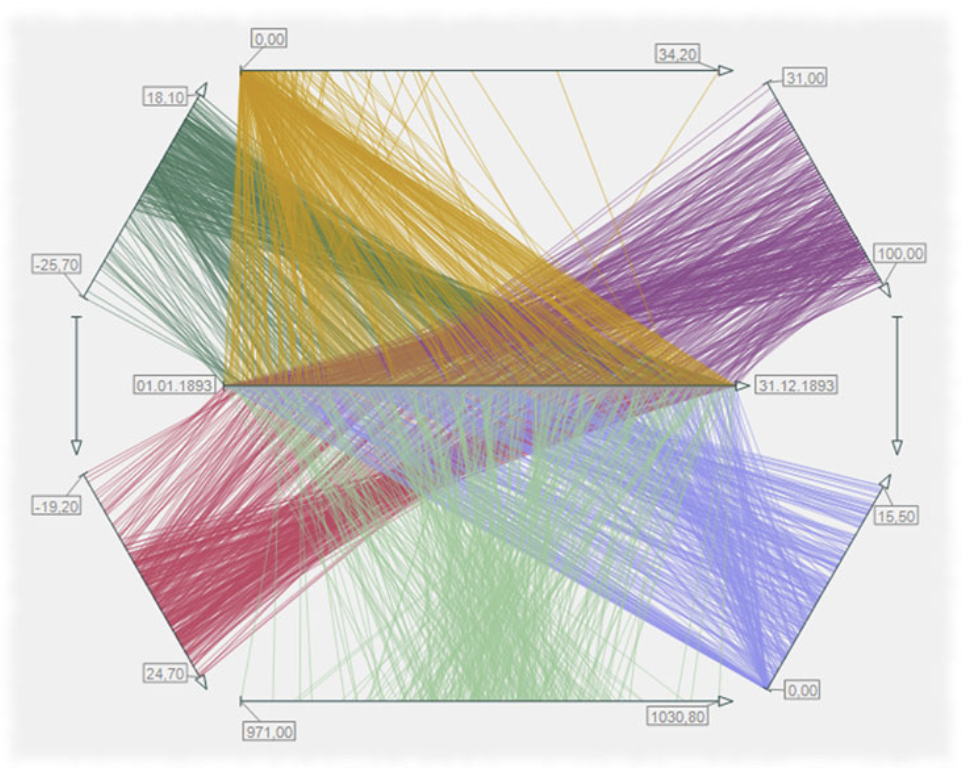
\includegraphics{src/images/TimeWheel}}
    \caption[Time Wheel]{Time Wheel. From  \cite{Aigner2011}.}
    \label{fig:timewheel}
\end{figure}\par


Four visualization techniques of geometric-projective techniques are limited in the maximum number of items. Consequently, \textit{multi-resolution CircleView, the Temporal Star and hierarchical techniques} are appropriate to visualize large amounts of data as shown in table \ref{table:GPscalability}. 

\begin{table}[H]
	\centering
	\caption[Scalability of \gls{GP}]{Scalability of \gls{GP}}
	\label{table:GPscalability}
	\begin{tabular}{lcc}
	\hline
	\gls{GP}-Technique & scalability \\
	\hline
	Flocking Boids & \cellcolor{red!25 }500 \\
	Kiviat Tube & \cellcolor{red!25 }20.000 \\
	MultiComb & \cellcolor{red!25 }10.000 \\
	Multi-resolution CircleView & \cellcolor{green!25 }$>$ 2mio.\\
	Parallel Glyphs &  \cellcolor{yellow!25 }15.000 - $>$ 1mio.\\
    Temporal Star &  \cellcolor{green!25 }$>$ 2mio.\\
	TimeWheel & \cellcolor{red!25 }10.000\\
	\hline
	\end{tabular}
\end{table}


In summary, only a few techniques are able to represent billions of data points. In the end most of them are limited through the screen pixels of the 2D-screen. 

In order to present large data effectively the visualization step alone in the visualization pipeline in \ref{fig:vispipeline} is not sufficient for scalable visualization. Preprocessing in the form of data reduction and data manipulation such as interaction techniques are required. Furthermore, aggregation methods such as multi-resolution (\ref{multi-resolution}) are promising techniques. These methods are also called advanced visual metaphors. 


\section{Analytical Techniques}\label{analytical}
In comparing the visualization techniques in \ref{vis} it was found that only a few techniques scaled beyond two million pixels. Thus, the need for data reduction becomes obvious. There are two ways of data reduction: to reduce data horizontally or vertically. 
Vertical data reduction describes the process of removing data rows (figure \ref{fig:vertical}) whereas horizontal data reduction (figure \ref{fig:horizontal}) is used for dimensionality reduction.

% \begin{figure}[H]
%     \centering
%         \scalebox{.1}{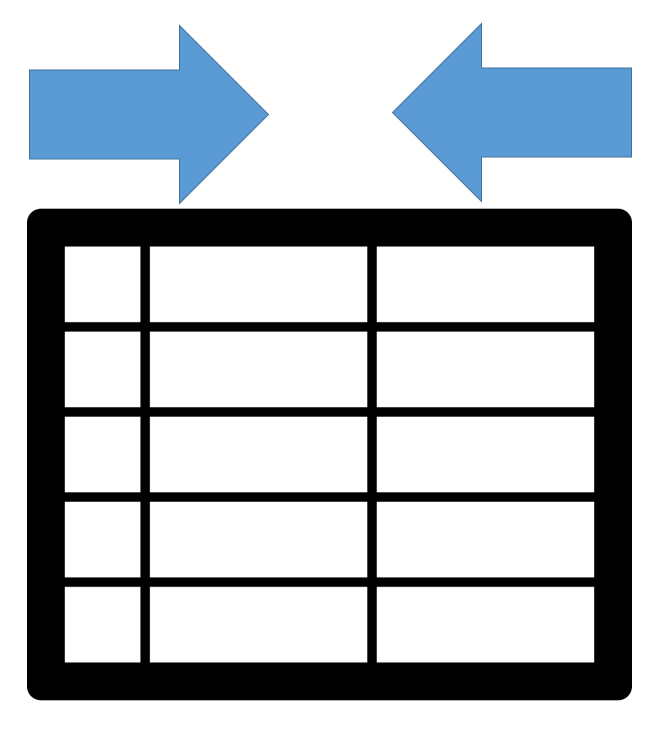
\includegraphics{src/images/dimreduce}}
%     \caption{Horizontal Data Reduction}
%     \label{fig:horizontal}
% \end{figure}

% \begin{figure}[H]
%     \centering
%         \scalebox{.1}{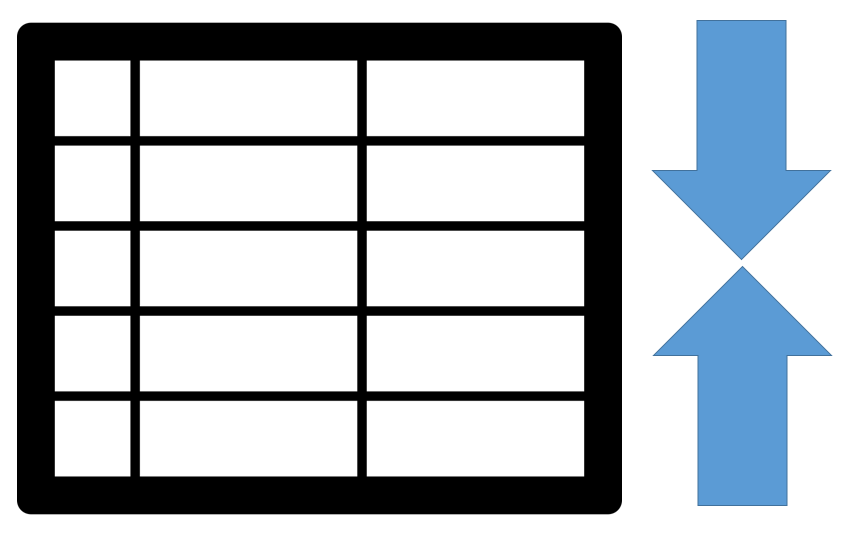
\includegraphics{src/images/aggregation}}
%     \caption{Vertical Data Reduction}
%     \label{fig:vertical}
% \end{figure}

\begin{figure}[H]
 \centering
         \subfloat[ Vertical Data Reduction]{\label{fig:vertical}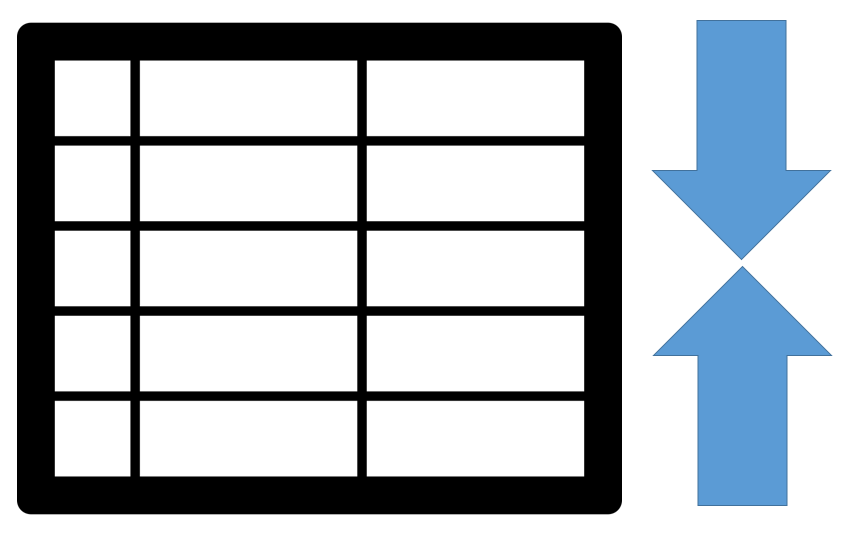
\includegraphics[width = 0.39\textwidth]{src/images/aggregation}}
\qquad
\qquad
        \subfloat[ Horizontal Data Reduction]{\label{fig:horizontal}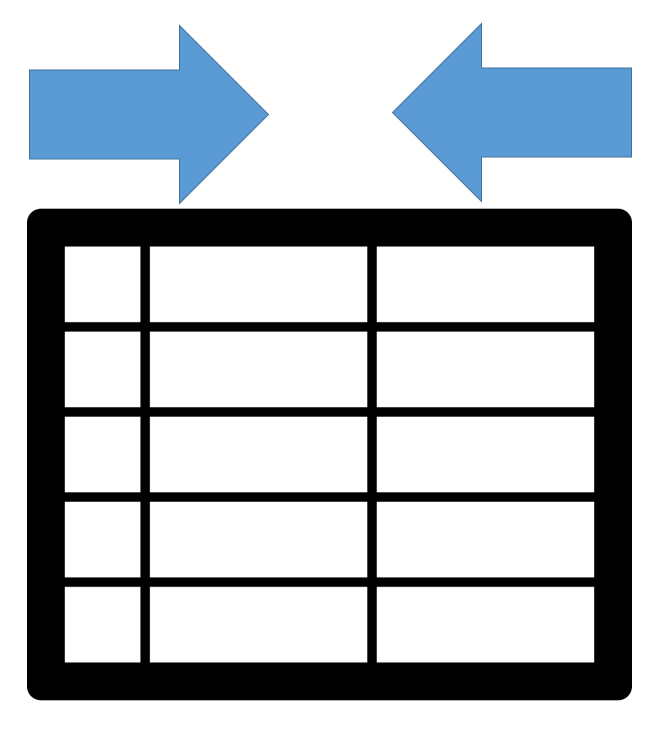
\includegraphics[width = 0.3\textwidth]{src/images/dimreduce}}
\end{figure}

\subsection{Vertical data reduction}
One way to decrease the size of large or huge data sets is to remove data rows. This section lists several data removal techniques. 

%One important issue for every technique is the question which data to keep and which data to remove. The disadvantage of data reduction is the information loss.
\textbf{Sampling \& Filtering: }\label{sampling}\label{filtering}
Sampling describes a strategy to reduce data by creating a subset of the original data. Sampling is scalable, reduces clutter, preserves information of the kept data as well as patterns and trends \cite{PiringerHarald2011}. Still, sampling may eliminate outliers or single data items and does not provide any guarantee to avoid visual overlap. \par
Filtering is a method to reduce data by specific criteria. With respect to visualization, filtering is often based on user input such as dynamic query sliders in the frontend. In the backend, filtering can also be applied to define data extracts. In both cases filtering can support the user in excluding task-irrelevant data portions and unlike sampling filtering may be appropriate to detect outliers. However, as filtering is based on the exclusion of irrelevant attributes it does not guarantee a specific target size of the data set. In some cases the target size might still be too large. Moreover, filtering also does not secure the discrimination of distinct data items  \cite{PiringerHarald2011}.\par
\textbf{Aggregation: }\label{aggregation}
Aggregation describes the process of grouping similar data items together. Aggregation methods can either aggregate data inside the data set or inside the visualization. Examples for data set aggregation are calculated dimensions which join multiple dimensions into a new one. Examples for visualization aggregation are clustered markers. The data set aggregation is discussed in section \ref{analytical} and visualization aggregation in section \ref{advancedmetaphor}.
Inside the data set aggregation reduces the data items. Even non-scalable visualization techniques can then display the aggregated data set.   Hierarchical, binned, pixel-aware and M4 aggregation are possible algorithms for aggregation.  
Temporal aggregation reduces the data size with respect to the time-specific characteristics. Data is aggregated according to the time unit (day, month, year) in temporal hierarchy levels. Examples for temporal aggregation are hierarchical axes  \cite{Chung2014}, which enable the user to navigate time. 
In visualization tools, aggregation is achieved by calculated fields which take dimensions from the data set as input and combine them with an equation into a new dimension.
% Temporal aggregation
\par
\textbf{Temporal Data Abstraction: }\label{temporalabstraction}
Temporal Data Abstraction  \cite{Aigner2011} reduces the number of data rows by focusing on relevant concepts, patterns, shapes over time and neglecting irrelevant details. Clusters and summary statistics  \cite{PiringerHarald2011} are typical examples for data abstraction. In the context of time-oriented data however, the authors found a trade-off between abstraction and accuracy: with low abstraction and a high accuracy the problem of cluttering occurs. 
One way to implement temporal data abstraction is to use natural language processing in visualization tools. The tool \textit{Answerrocket} implemented an NLP-Approach connected with visualization. Another way to achieve data abstraction is the use of unsupervised machine learning methods, such as clustering.
Clustering as defined in the user tasks \ref{tasks} as \textbf{T2} has the advantage of reducing visual clutter by displaying the natural groups of the data instead of every single data item. It also preserves patterns and outliers if the similarity measure is appropriate.
Moreover, data abstraction can also be achieved by simplifying the pattern's shape. In order to simplify a visualization relevant data items are kept while irrelevant data items are removed. Temporal Data Abstraction in tools can be implemented by any method which keeps the characteristic shape, i.e. by assigning relevance to data items, and by any method which removes data points. \par

Other ways to reduce data vertically are binning and pivoting. We will not explain them here in detail as they apply to continuous and hierarchical data sets which are beyond our scope. 

\subsection{Horizontal data reduction}
Besides data removal data size can be reduced by decreasing data dimensionality. Since business data often is multi-dimensional but visualization techniques are limited in the number of attributes dimensionality reduction is a way to process data sets in a way so that they can be displayed by visualization techniques. \par
\textbf{Dimensional Reduction:} The advantage of dimension reduction techniques such as \gls{PCA} or \gls{SOM} is that they keep the distance between two points after the projection. Thus, anomalies can be detected and the user can be supported with his tasks \textbf{T6}.
\par
\textbf{Calculated Dimensions: }Dimensions can also be reduced by aggregated dimensions which are also known as calculated dimensions. Instead of visualizing the original dimensions multiple dimensions can be combined.
\par

In short, data reduction techniques such as horizontal and vertical data reduction condense  data sets in order to fit data sets on the screen and overcome the problem of visual clutter. With data reduction, non-scalable visualization techniques can be used. 

\subsection{Data modeling \& pattern search}\label{patternsearch}
Next to data reduction techniques, \textit{data modeling} techniques are an important feature for tools. They enable the user to find patterns in the data and thus, support the user in the user tasks \textbf{T2, T3, T5, T6}. Data Modeling covers clustering, classification, network modeling and predictive modeling \cite{Zhang2001}. 
\par
Besides data reduction, \textit{pattern search} is an important feature in navigating a large data set. Given a defined pattern, similar patterns are retrieved. One implementation of pattern search are \textit{Timeboxes}  \cite{Buono2005}. With timeboxes the user can drag out a rectangle which defines the pattern. Then similar patterns are queried and retrieved. That is why pattern search supports the user in the user tasks \textbf{T1} and \textbf{T7} by detecting regions of interest and supporting in navigation. In large data sets pattern search is required more than ever as the human perception is not able to perceive patterns in large data sets anymore.


\section{Advanced Visual Metaphors}\label{advancedmetaphor}
Another way to implement aggregation (\ref{pattern}) are advanced visual metaphors. Visual metaphors define how data is mapped to geometric primitives. The mapping function that is used influences visual scalability. The visual metaphor of pixel-oriented techniques maps each data item to one pixel. Hence, the maximum number of displayed pixels is equal to the number of screen pixels. The visual metaphor of bar charts  arrange data items as bars along the monitor width ($w$). If each bar would have the width of one pixel, a bar chart could only visualize  $w$ data items. Thus, the visual metaphor limits how many data items can be showed at most. Advanced visual metaphors can enhance the scalability of visualization techniques  \cite{Eick2002}. \par
 \textbf{Multi-resolution:} \label{multi-resolution} one way to improve visual metaphors are multi-resolution metaphors  \cite{Keim2005}. The idea of multi-resolution is to show more relevant data items at a pixel-based level and less relevant data items in an aggregated manner. Therefore, relevance is assigned to each data point and then data points are aggregated according to their relevance. Less relevant data are condensed to larger clusters while more relevant data have smaller clusters. Then the clusters are mapped to the screen space. Thus, the resolution denotes the ratio of data items compared to screen pixels. Pixel-oriented techniques have a resolution of 1:1 as they map one data item to one pixel. With multi-resolution it is possible to extend the pixel-limit of $w*h$ for larger data sets. 
 \begin{figure}
     \centering
     \scalebox{0.5}{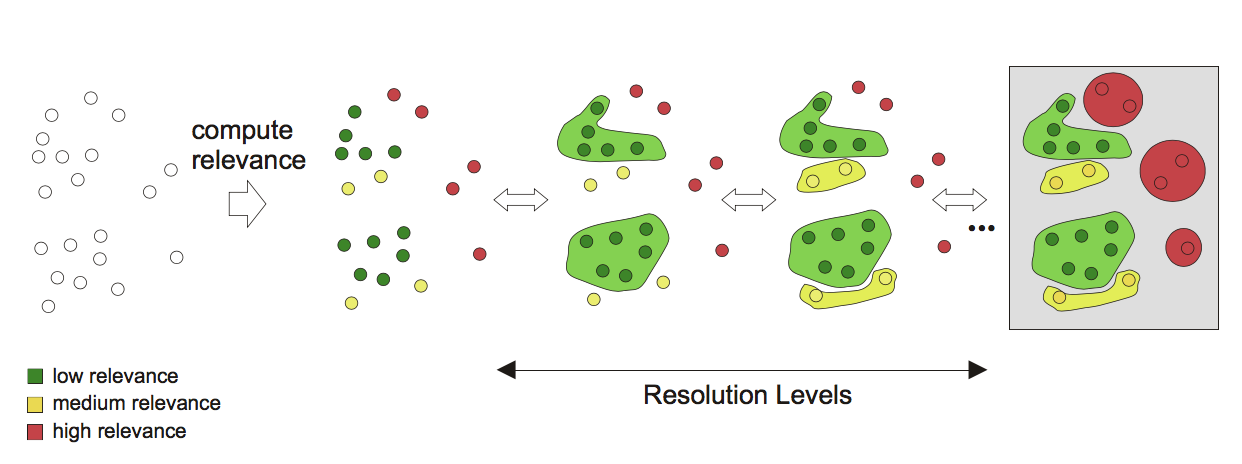
\includegraphics{src/images/multi-resolution}}
     \caption[Multi-resolution]{\textit{Multi-Resolution: }data items are grouped with variying granularity depending on their relevance. From  \cite{Keim2005}}
     \label{fig:multi-resolution}
 \end{figure}
 In a multi-resolution visualization the resolution is usually less granular at the \textit{Overview-Level} and more granular at the \textit{Detail-Level} (compare \ref{fig:multi-resolution}). \textit{CircleView} is one visualization technique with a multi-resolution metaphor. Multi-resolution is one important aspect for visualization tools to improve visual scalability.\par
\textbf{Aggregation Markers:}\label{aggregationmarkers} A different approach for advanced visual metaphors are aggregation markers (also known as point clustering). Point clustering groups a larger set of data points onto a smaller set in the 2D-plane  \cite{Morrison2014}. This process decreases the visual overlap of data points and thus, increases the perception of large data sets. Moreover, point clustering accelerates the rendering process by first rendering the data clusters  and later loading more detailed data items. This incremental loading generates user satisfaction by shorter response times.\par
In contrast to data reduction methods advanced visual metaphors are not actually decreasing data size. They only decrease the \textit{perceived data volume} and keep the actual data volume. This differentiates methods like multi-resolution and aggregation markers from methods like data reduction. 


\section{Interaction Techniques}
Interaction Techniques describe how the user can interact with the data. In this section interaction techniques for large data sets are discussed and how they can enhance scalability. As discussed in \ref{problems} challenges in visualization are pixel overlap, limited screen space, identifying a region of interest and navigation. Interaction techniques can overcome these problems. 
\par
Overlap can be eliminated by \textit{drill-down functions} such as filters and zoom, which reduce the displayed data and hence, minimize the overlap. \par
\textbf{Filtering:} With filters a set of variables can be selected and the visualization is only showing the respective variables. The excluded data items are kept in memory.
One way of filtering is the use of dynamic queries. A specific dynamic query for time-oriented data is the use of time-boxes \cite{Hochheiser2004}. These boxes are rectangular selection areas which are drawn by the user. The tool then only displays values with a similar pattern to the pattern in the time-boxes.\par
\textbf{Zooming} is the way of drilling down into a data set to a lower level of detail. The user focus is shifted from the Overview-Level to a Detail-Level where the displayed data is reduced and thus, overlap decreased. One special way of zooming is semantic zooming  \cite{Boulos2003}. Instead of zooming, multiple linked views are preferred for a higher number of displayed objects.
\par

The limited screen space can be enhanced by \textit{interactive distortion techniques} such as \textbf{fish-eye, bifocal displays} and \textbf{perspective walls}. The advantage of distortion techniques is their support in focus and context. Subsets can be analyzed at a detail-level while less relevant data is shown in a comprised manner. By providing focus and context, distortion techniques help the analyst in navigating through large data sets. Since data is aggregated but not removed, distortion techniques are good for finding outliers. One disadvantage is that the user may misinterpret distances because of the distortion.
\par

\label{navigation}
Closely related to interaction techniques are appropriate \textit{interactive navigation techniques},  such as linked views and information murals (also known as navigational maps) which allow the user for navigating inside the data set \cite{Jerding1998}. With linked views the user can see different level of detail in one glance and navigate though different level of detail with navigational maps. Navigation also helps in finding a region of interest.
The differentiation between navigation and interaction techniques is not selective.
\label{zoomingVsmultiple}
Ware  showed in figure \ref{fig:zoomVsMultiWindow} that zooming is an easy-to-use-tool for a small amount of items \cite{Ware2012}. However, if the user needs to keep three items or more in visual working memory, then multiple windows are more effective than zooming. Thus, displaying large time-oriented data requires a layout with multiple simultaneous views if the number of data objects exceeds three items. Multiple coordinated views are called linked views. Often, linked views are combined with Brushing. \par

\textbf{Brushing \& Linking }is one way to achieve \textit{focus and context} but it also supports the user with the user task \textbf{T3} as similar items are highlighted. Moreover, in the context of time-oriented data a typical brushing activity is the selection of a smaller time-span to see more details during this period of time. 
\par

\begin{figure}[H]
    \centering
        \scalebox{.5}{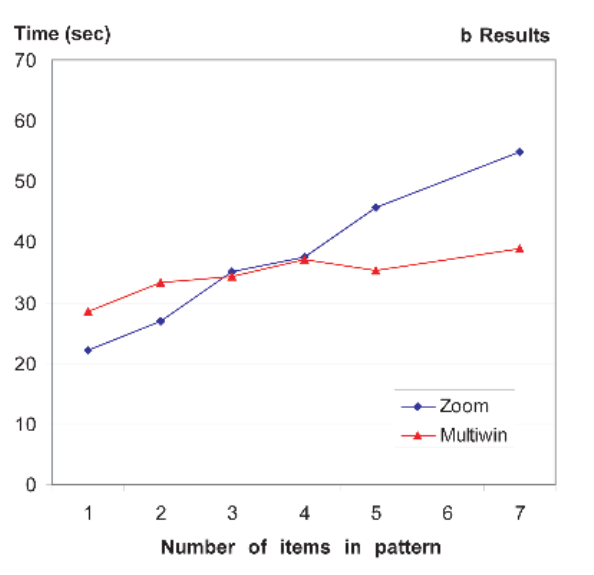
\includegraphics{src/images/zoomVSmultiWindow}}
    \caption[Comparison of Zoom and Multiple Linked Views]{Measured task performance of zooming compared to multiple windows.  \cite{Ware2012}}
    \label{fig:zoomVsMultiWindow}
\end{figure}

Another navigation technique for large data sets is the use of \textbf{navigational maps}.\par
\textbf{Navigational Maps:} display the complete data set next to other linked views as a miniature version in a separate window. With this method the user can see the data set in detail as well as keep the context and navigate through the data set.\par
\textbf{Search: }\label{search} Besides navigational maps \textit{Searching} navigates inside the data set. Since large data sets are difficult to overview, unaided the user might not find regions of interest. Instead, searching the data set supports the analyst. Searching uses natural language processing (NLP) to retrieve queries from the backend. Some tools have started to include visualizations in the search area. That way, the analyst can search visualizations for patterns, trends, specific points in natural language. 
\par

The discussed interaction techniques are only a subset of available interaction techniques. We focused on interaction styles which can solve the problems of large data visualization and thus enhance visual scalability. We assume that interaction is in the responsibility of the visualization tools.

% \begin{table}[H]

%     \begin{tabular}{|l| l l l|}
%         \hline
%             &                   & 1 & 2\\
%         \hline
%             &                   & \begin{turn}{90} Multi-Resolution\end{turn}   & \begin{turn}{90} Aggregation\end{turn}\\
%         \hline
%         A   & avoids overlap    & \checkmark                                    &\\
%         B   & keeps spatial information     & x                                 &\\
%         C   & can be localised  & \checkmark                                    &\\
%         D   & is scalable       & \checkmark                                    &\\
%         E   & is adjustable     & x                                             &\\
%         F   & can show point/ line attribute    & x                             &\\
%         G   & can discriminate points/ lines    & x                             &\\
%         H   & can see overlap density           & x                             &\\
%         \hline
%     \end{tabular}
% \end{table}

\section{Success Criteria for Large Scale Data Visualization}\label{success}
After our analysis of the limiting factors for displaying large data sets we come to the conclusion that effective visualizations for large data sets combine scalable visualization techniques, data reduction methods and interaction techniques. The question is \textit{not} how many pixels can be displayed by a visualization technique but whether the visualization technique allows the user for perceiving patterns. In large data sets, visualization techniques that support pattern perception are techniques that display data effectively. Hence, they scale to large data. Techniques which scale to large data sets are called advanced data visualization (\gls{ADV}). In summary, visualization tools should integrate (\gls{ADV}) to visualize time-oriented multivariate data. 

Moreover, pattern supporting visualizations are achieved by the use of \textit{appropriate visual metaphors} and \textit{data reduction methods}. Data reduction methods can aggregate overlapping data items to cluster by either mapping data density to color or by displaying the mean and the range of data. Visual Metaphors include techniques such as multi-resolution which enhance the number of pixels that can be displayed. Data and dimension reduction reduces the number of data items which need to be displayed. Thus, even non-scalable visualization techniques can display the reduced data. 
\par

Bringing all findings together, the important factors for the visualization of large data sets to support decision-making are the following: 
\begin{enumerate}[noitemsep]
\item How are advanced visualization techniques integrated? 
\item How is data reduction achieved? 
\item How are aggregation metaphors implemented? 
\item How are interaction techniques supported?
\end{enumerate}

Visualization tools need to offer solutions to these questions for a successful visualization of large data sets. Thus, we propose the following success criteria for large data visualizations and define a best possible implementation. This definition will be equivalent to the best score for completeness of the scoring model in chapter \ref{chap:Tools}.
\begin{enumerate} [noitemsep]
\item Analytical Techniques 
\begin{enumerate}
    \item The tool offers horizontal data reduction.
    \begin{itemize}
        \item Let $k$ be the desired number of dimensions. A data set can be reduced to $k$ dimensions. The visualization takes $k$ dimensions as input.
        \item Dimensions can be aggregated and saved as a new dimension.
    \end{itemize}
    \item The tool offers vertical data reduction.
    \begin{itemize}
        \item Data sets can be reduced by omitting rows.
        \item Filters are offered to interactively reduce the number of shown data items.
        \item Data points can be removed from data set. 
        \item Relevance can be assigned to data points so that important data points can be kept and less relevant data points can be removed.
        \item Data items can be clustered and saved.  
    \end{itemize}
    \item The tool offers data modeling options.
    \item The tool offers pattern search.
\end{enumerate}


\item Visualization Techniques
\begin{enumerate}
\item The tool offers all possible visualization techniques.
\item Every visualization technique can cluster or aggregate data items.
\item Every visualization technique can use multi-resolution.
\end{enumerate}

\item Interaction Techniques
\begin{enumerate}
\item The tool offers the drill-down functions zoom and filter for every visualization.
\item The tool offers the distortion techniques fish-eye, perspective wall, bifocal display for every visualization.
\item The tool offers the navigation techniques navigational maps, coordinated windows, searching for every visualization.
\end{enumerate}

\end{enumerate}
